\documentclass[border=10pt]{standalone}
\usepackage{pgfplots}
\pgfplotsset{compat=1.17}
\definecolor{myblue}{RGB}{0,0,255}
\definecolor{myred}{RGB}{255,0,0}
\definecolor{mygreen}{RGB}{0,128,128}
\definecolor{myorange}{RGB}{255,165,0}
\definecolor{mypurple}{RGB}{128,0,128}

\begin{document}
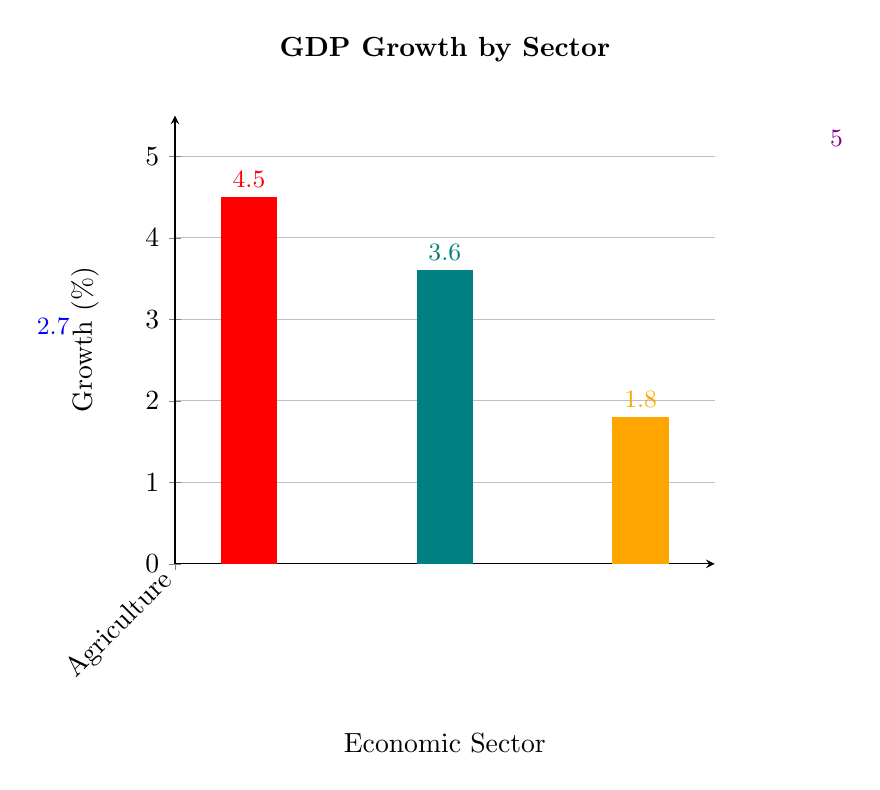
\begin{tikzpicture}
\begin{axis}[
    ybar,
    enlargelimits=0.15,
    legend style={at={(0.5,-0.15)},
    anchor=north,legend columns=-1},
    ylabel={Growth (\%)},
    symbolic x coords={Agriculture, Industry, Services, Construction, Technology},
    xtick=data,
    nodes near coords,
    nodes near coords align={vertical},
    title={\textbf{GDP Growth by Sector}},
    title style={font=\bfseries},
    every axis plot/.append style={fill},
    bar width=20pt,
    grid=none,
    axis lines=left,
    ymajorgrids=true,
    ymin=0,
    ymax=5.5,
    ytick={0,1,2,3,4,5},
    xticklabel style={rotate=45,anchor=east},
    xlabel={Economic Sector},
    xlabel style={yshift=-10pt},
    ylabel style={yshift=10pt},
    title style={yshift=10pt},
    every node near coord/.append style={font=\small},
    ]
    \addplot[myblue] coordinates {(Agriculture,2.7)};
    \addplot[myred] coordinates {(Industry,4.5)};
    \addplot[mygreen] coordinates {(Services,3.6)};
    \addplot[myorange] coordinates {(Construction,1.8)};
    \addplot[mypurple] coordinates {(Technology,5.0)};
\end{axis}
\end{tikzpicture}
\end{document}